\begin{multicols}{2}
\textbf{Ingredients}
\begin{itemize}
\item 2 lbs peeled \& deveined shrimp 
\item 1 yellow onion (diced)
\item $\sim 6$ cloves of garlic (minced)
\item 2 cups rinsed and drained quinoa
\item 1 box (32 oz) chicken stock
\item 3 tbsp olive oil  
\item 1.5 tsp chili powder
\item 1 tsp cayenne 
\item 1 tsp garlic powder
\item 1 tsp onion powder 
\item 1 tsp of salt to cook shrimp and more to taste
\item the juice of 1 lemon and more to taste 
\item 3 tsp parsley flakes 





\end{itemize}


\columnbreak
\textbf{Procedure:}
\medskip


\begin{enumerate}
\item In a large pan, cook shrimp in 2 tbsp olive oil, chili powder, salt, and cayenne until pink. Remove from pan and set aside. Sautee garlic and diced onion in pan in another tablespoon of olive oil until onions are translucent. 

\medskip

\item At the same time start oven roasting or steaming brussels sprouts. 

\medskip

\item Add chicken stock and rinsed quinoa to pan and bring to a boil. Reduce to medium low heat until quinoa is cooked and add shrimp, garlic powder, onion powder, and lemon juice to taste. 



 
\end{enumerate}

\end{multicols}



%\begin{center}
%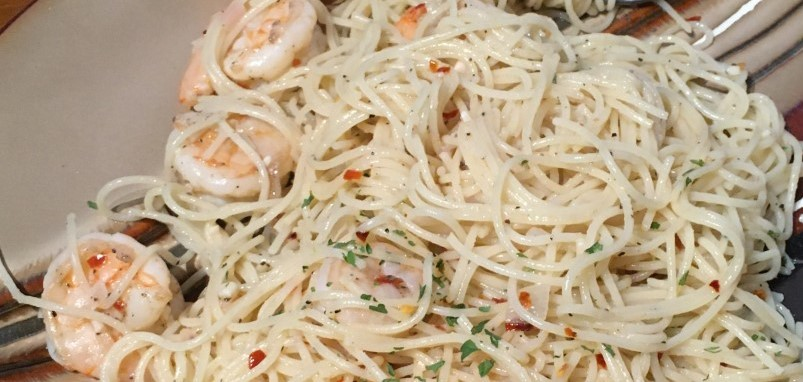
\includegraphics[scale=0.65]{Pasta/Shrimp Scampi/Shrimp Scampi.jpg}
%\end{center}